\subsection{Data sets}
Photon data with a newest version of events reconstruction (would be last version) from \textit{Fermi}-LAT
\begin{itemize}
    \item P8R2\_ULTRACLEANVETO\_V6 data from 07/08/2008 to 16/10/2017 ($\sim$9 years)
    % \item Use weekly data file from week 10 to week 399 ($\sim$ 7 years)
    \item Collect photon energy range = 10 GeV to 1 TeV
    \item $\theta_{\text{NADIR}} = 68.4^\circ - 70^\circ$(Earth’s limb) 
    \item Use $\theta_{\text{LAT}} < 70^\circ$
\end{itemize}
Note that the reasons that we use ULTRACLEANVETO type of event reconstruction are it is the cleanest reconstruction catalogue.

\subsection{Flux extraction}
\begin{enumerate}
    \item Make 2D histograms with 25 bins per decade of energy
    \item Select photon data and fill in the 2D histograms
    \item Calculate exposure maps which include the effective area and livetime of the LAT as it observed the Earth
    \begin{equation}
      \textbf{Flux} \equiv \frac{dN_\gamma}{dE} = \frac{\int_{\text{Limb region}}(\text{Count map}/\text{Exposure map})}{\Delta\Omega\Delta E }
    \end{equation}
    % \item Reprocess photon data by taking into account
    %     \begin{itemize}
    %         \item Treat photon energy bias 3.7\% that be affected the energy range above 10 GeV
    %         \item Adjust $\theta_\text{N}$ due to LAT altitude shift due to detection of $\theta_{\text{Limb}}$ was tilt relatively to altitude of the spacecraft when orbit around asymmetric spherical Earth 
    %     \end{itemize}
    % \item Construct 2D histogram in Earth's angular coordinate ($\theta_{\text{ZENITH}}$ and $\phi_{\text{EARTH}}$)
    % \item Fill photon data in different energy range
    % \item Calculate exposure maps which include effctive area and time that LAT field of view can glimpse area of interest
    % \item Divide every single grid count map by exposure map
    % \item Sum over limb region of this map then divided by solidangle and energy bin width, then fill data in $\gamma$-ray energy spectrum as the formula 3.1
    % \begin{equation}
    %     \text{Flux}\equiv\frac{dF}{dE} = \frac{\int_{\text{Limb region}} (\text{Count map}/\text{Exposure map})}{\Delta\Omega\Delta E}
    % \end{equation}
    \item Taking consider background subtraction from a average uniform background photon distribution by treating bin by bin 
\end{enumerate}


%---------------------------
% Coordinate transformation
%---------------------------
\subsection{Coordinate Transformations}


\begin{figure}[h!]
    \centering
    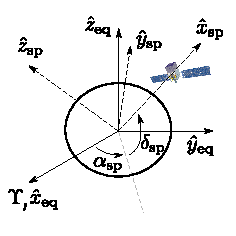
\includegraphics[width=0.5\textwidth]{img/fig_coordinate/coord_eq_sp.pdf}
    \caption{Coordinate transform between celestial and spacecraft}
\end{figure}

\begin{equation}
    \begin{split}
    \hat{x}_\text{sp} &= \cos\delta_\text{sp}\cos\alpha_\text{sp}\hat{x}_\text{eq} + \cos\delta_\text{sp}\sin\alpha_\text{sp}\hat{y}_\text{eq} + \sin\delta_\text{sp}\hat{z}_\text{eq}\\
    \hat{z}_\text{sp} &= - \sin\delta_\text{sp}\cos\alpha_\text{sp}\hat{x}_\text{eq} - \sin\delta_\text{sp}\sin\alpha_\text{sp}\hat{y}_\text{eq} + \cos\delta_\text{sp}\hat{z}_\text{eq} \\
    \hat{y}_\text{sp} &= \hat{z}_\text{sp} \times \hat{x}_\text{sp}
    \end{split}
    \label{eq:tf_eq_sp}
\end{equation}

The transform matrix between equatorial coordinate and spacecraft coordinate could be represented as a relation in Eq \ref{eq:tf_eq_sp}

\begin{equation}
    \hat{r}_\text{sp} \equiv T_{\text{eq}\rightarrow\text{sp}} (\delta_\text{sp}, \alpha_\text{sp}) \hat{r}_\text{eq}
\end{equation}

\begin{equation}
    \begin{split}
    \hat{x}_\text{p} &= \cos\delta^\text{x}_\text{p}\cos\alpha^\text{x}_\text{p}\hat{x}_\text{eq} + \cos\delta^\text{x}_\text{p}\sin\alpha^\text{x}_\text{p}\hat{y}_\text{eq} + \sin\delta^\text{x}_\text{sp}\hat{z}_\text{eq}\\
    \hat{z}_\text{p} &= \cos\delta^\text{z}_\text{p}\cos\alpha^\text{z}_\text{p}\hat{x}_\text{eq} + \cos\delta^\text{z}_\text{p}\sin\alpha^\text{z}_\text{p}\hat{y}_\text{eq} + \sin\delta^\text{z}_\text{sp}\hat{z}_\text{eq}\\
    \hat{y}_\text{p} &= \hat{z}_\text{p} \times \hat{x}_\text{p}
    \end{split}
    \label{eq:tf_eq_p}
\end{equation}

According to Eq \ref{eq:tf_eq_p}, the transformation matrix between LAT-boresight and equatorial coordinate could be derived from
\begin{equation}
    \hat{r}_\text{p} \equiv T_{\text{eq}\rightarrow\text{p}} (\delta^\text{x}_\text{p}, \alpha^\text{x}_\text{p}, \delta^\text{z}_\text{p}, \alpha^\text{z}_\text{p}) \hat{r}_\text{eq}
\end{equation}

\begin{figure}[h!]
    \centering
    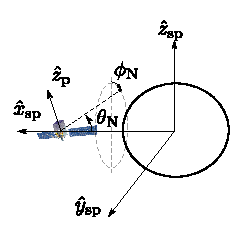
\includegraphics[width=0.5\textwidth]{img/fig_coordinate/coord_eq_p.pdf}
    \caption{Coordinate transform between spacecraft and nadir angle}
\end{figure}

Importantly, the current status of lat field of view need to be consider in order to fill in the exposure map with the Earth’s polar coordinate from satellite point of view as 

\begin{equation}
    \hat{r}^\text{o}_\text{sp} (\theta_\text{N}, \phi_\text{N}) \equiv -\cos\theta_\text{N}\hat{x}_\text{sp} + \sin\theta_\text{N}\cos\phi_\text{N}\hat{z}_\text{sp} + \sin\theta_\text{N}\sin\phi_\text{N}\hat{y}_\text{sp}
    \label{eq:def_r0}
\end{equation}

Since the spacecraft coordinate has already linked to the nadir's angle, the next step is to transform it into central coordinate which basically is the equatorial coordinate and convert it into LAT-boresight coordinate (Eq \ref{eq:def_r0_to_rp})

\begin{equation}
    \hat{r}^\text{o}_\text{p} (\theta_\text{N}, \phi_\text{N}) = T_{\text{eq}\rightarrow\text{p}} (\delta^\text{x}_\text{p}, \alpha^\text{x}_\text{p}, \delta^\text{z}_\text{p}, \alpha^\text{z}_\text{p}) \left[T_{\text{eq}\rightarrow\text{sp}} (\delta_\text{sp}, \alpha_\text{sp})\right]^{-1} \hat{r}^\text{o}_\text{sp} (\theta_\text{N}, \phi_\text{N})
    \label{eq:def_r0_to_rp}
\end{equation}

\begin{figure}[h!]
    \centering
    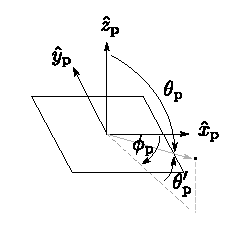
\includegraphics[width=0.5\textwidth]{img/fig_coordinate/coord_plane.pdf}
    \caption{Detector's boresight in cartesian and polar coordinate}
    \label{fig:tf_lat_pol_car}
\end{figure}

Geometrically, angular coordinate of LAT plane could be obtained from normalized component of the cartesian unit vector as in Fig \ref{fig:tf_lat_pol_car}.
The exposure accumulation has been calculated in every single grid from the previous relation.

The calculation of exposure map has to be done wisely one energy at a time
due to the effective area of the spacecraft at each angle has various efficientcy depends on the incident energy of gamma-ray as in the Fig \ref{fig:lateff}.
Under the condiiton of exposure-energy at a time, another factor that has to be consider carefully is the resolution of the exposure map.
The higher resolution, the longer calculation time consumption which means we have to make $\theta_\text{N}$ more precise than $\phi_\text{N}$ because the limb region is more sensitive.

\begin{figure}[h!]
    \centering
    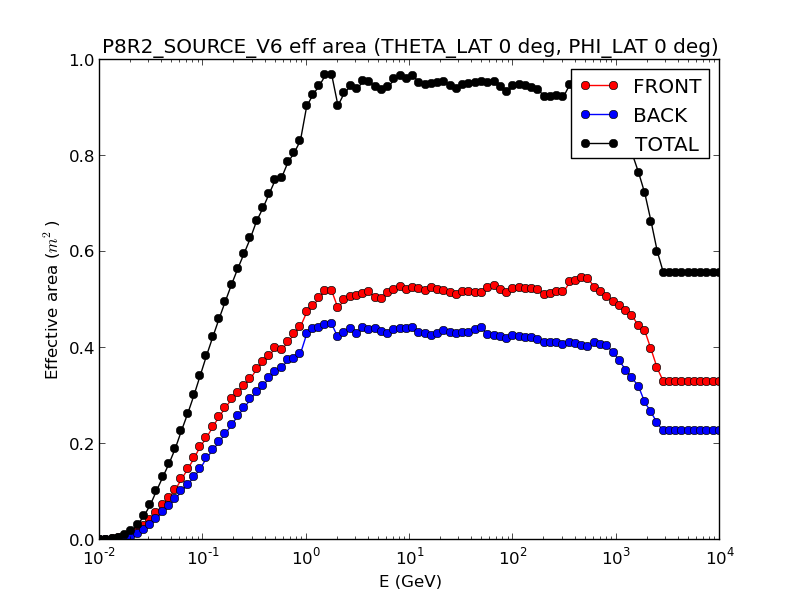
\includegraphics[width=0.8\textwidth]{img/eff_energy_dist}
    \caption{Effective area of \text{Fermi}-LAT}
    \label{fig:lateff}
\end{figure}

For both reasons, the first version of calculation takes approximately a month or more to finish.
However, there is a plenty of room to improve. Here is why parallel computation fit really well to this problems.
To maximize all of the threading process in the cluster, master-slave technique has been applied to get rid of the idle thread to maximize our resource of computation.

%--------------------------
%     Interaction Model
%--------------------------

\subsection{Interaction model}
Incident proton spectrum in rigidity be represented as \\
\textbf{Single power law (SPL)}
\begin{equation}
    \frac{dN}{dR} = R_0R^{-\gamma}
    \label{eq:spl}
\end{equation}
\textbf{Broken power law (BPL)}
\begin{equation}
\frac{dN}{dR}=
  \begin{cases}
    R_0R^{-\gamma_1}\ :\ E < E_{\text{Break}}\\
    R_0[R(E_{\text{Break}})]^{\gamma_2-\gamma_1}R^{-\gamma_2}\ :\ E \ge E_{\text{Break}}
  \end{cases}
  \label{eq:bpl}
\end{equation}

In this work, we use the scattering amplitude from hadronic collision \cite{K&Omodel} that could produce a photon as a secondary product that could be detected by \textit{Fermi}-LAT.
\begin{equation}
    \frac{dN_\gamma}{dE_\gamma} \propto \int^{E_{\text{max}}}_{E_\gamma} dE'\frac{dN_p}{dE'} \frac{d\sigma^{pp\rightarrow\gamma}(E',E_\gamma)}{dE_\gamma}
\end{equation}
\par The atmospheric composition already known well enough that mostly combined with nitrogen gas as well as oxygen molecules \cite{atmosCompos}. 
In order to get scattering amplitude from proton-proton collision we treat a crossection of single hadronic collision with a fraction of nitrogen atom which is almost equal to oxygen atom \cite{WAtwater} at relativistic level of kinetic energy.
\par In 2015, the direct measurement of Helium specrtum has been done by using AMS-02 in \cite{AMS-02Helium}. Improvement of model precision was included by taking into account incident of Helium cosmic ray particle as a first order correction and please note that we ignore other heavier atom.

\begin{equation}
    \frac{dN_{\gamma}}{dE_\gamma}(E_\gamma) \propto \sum_{E_{\text{inc,i}}}\left[\frac{E_{\text{inc,i}}}{E_{\gamma}}\Delta(E_{\text{inc,i}}) \right]\left[ f_{pp}\textcolor{red}{\frac{dN_\text{H}}{dE_{\text{inc}}}(E_{\text{inc,i}})}\left\{ 1+\textcolor{olivegreen}{\frac{\sigma_{\text{HeN}}}{\sigma{pN}}}\left(\textcolor{red}{\frac{dN_{\text{H}}}{dR}}\right)^{-1} \textcolor{blue}{\frac{dN_{\text{He}}}{dR}} \frac{dR_{\text{He}}}{dR_{\text{H}}}  \right\}\right]
\end{equation}

where
\begin{itemize}
    \item Red color terms is an \textcolor{red}{incident proton spectrum} as in Eq (\ref{eq:spl}, \ref{eq:bpl})
    \item \textcolor{blue}{Use helium spectrum from AMS-02 measurement (2015)}
    \item $f_{pp}\equiv E_\gamma(d\sigma^{ij\rightarrow\gamma}/dE_\gamma)$ is a table in K$\&$O model which behave like a scattering amplitude
    that depend on the energy of incident particle
    \item Crossection \textcolor{olivegreen}{$\sigma_{\text{HeN}}/\sigma_{pN}$} at energy more than 10 GeV is approximately plateau ($\approx 1.6$)
\end{itemize}


%--------------------------
%       Optimization
%--------------------------

\subsection{Optimization}

\par \textbf{Poisson likelihood function} define as Eq \ref{eq:likelihood}
\begin{equation}
    \mathcal{L} = \prod_{i=1}^{N} P_{\text{pois}}(n_{\text{i,model}}, n_{\text{i,measurement}})
    \label{eq:likelihood}
\end{equation}
Since our spectrum order is in different order of magniture, then the better way to define an objective function is to redefine a likelihood as a log-likelihood function for numerically convenient like Eq \ref{eq:loglikelihood}. 
\begin{equation}
    Sum = \sum_{i=1}^{N} -\log P_{\text{pois}}(n_{\text{i,model}}, n_{\text{i,measurement}})
    \label{eq:loglikelihood}
\end{equation}


\par In order to get a best fit spectral indices, we do an optimization with a proper trial parameters for take gradient descent from Poisson loss function between model spectrum and flux from measurement as Figure \ref{flow:optimize}


% Define block styles
\tikzstyle{decision} = [diamond, draw, fill=red!10, 
    text width=4.5em, text badly centered, node distance=3cm, inner sep=0pt]
\tikzstyle{block} = [rectangle, draw, fill=blue!10, 
    text width=7em, text centered, rounded corners, minimum height=4em]
\tikzstyle{longblock} = [rectangle, draw, fill=blue!10, 
    text width=10em, text centered, rounded corners, minimum height=4em]
\tikzstyle{line} = [draw,thick, -latex']
\tikzstyle{cloud} = [draw, ellipse,fill=red!20, node distance=3cm,
    minimum height=4em]

\begin{figure}[!h]
    \centering
    \begin{tikzpicture}[node distance = 10em, auto]
        \node [block, fill=black!10] (powerlaw) {powerlaw spectrum of proton in rigidity};
        \node [block, right of = powerlaw, node distance = 15em] (model) {$\gamma$-ray spectrum from model};
        \node [block, right of = model] (measurement) {$\gamma$-ray spectrum from measurement};
        \node [block, below left of = measurement, node distance = 12em] (pois) {Poisson likelihood function};
        \node [block, below of = powerlaw] (varyPar) {Apply gradient to parameters $\gamma$, $R_0$};
        \node [decision, below of = varyPar, fill = blue!10] (bestfit) {Best fit?};
        \node [block, right of = bestfit, node distance = 15em, fill = red!10] (return) {Return best fit parameters};

        \path [line] (powerlaw) -- node [anchor=south] {K\&O model} (model);
        \path [line] (model) -- (pois);
        \path [line] (measurement) -- (pois);
        \path [line] (pois) -- (bestfit);
        \path [line] (bestfit) -- node [anchor=east] {No} (varyPar);
        \path [line] (varyPar) -- (powerlaw);
        \path [line] (bestfit) -- node [anchor=north] {Yes} (return);
    \end{tikzpicture}
    \caption{Flow chart of optimization process}
    \label{flow:optimize}
\end{figure}

%--------------------------
%       Optimization
%--------------------------

\subsection{Monte Carlo Simulation}
In this section, we perform a brute force method to find an error of any parameters (spectral indices and break point energy). For a \textbf{statistical error (random error)}, we rerandom a counts on each bin by poisson random generator and recalculate the flux after that optimize it as the Fig \ref{flow:optimize} do.
The process of this algorithm has shown in Fig \ref{flow:montestat}.
The amount of simulation process require an enough number of sampling to fill up the optimized parameters and see the shape of gaussian distribution curve looks obvious enough which our work done is roughly 2000 sampling.

\begin{figure}[h!]
    \centering
    \begin{tikzpicture}[node distance = 12em, auto]
        \node [decision, fill = black!10, text width = 6em] (sampling) {While \\ sample $<$ N};
        \node [block, right of = sampling] (randStat) {Random raw count every bin by using Poisson function};
        \node [block, right of = randStat] (fluxcompute) {Calculate new $\gamma$-ray spectrum};
        \node [block, below of = fluxcompute, fill=yellow!10] (optimize) {Optimization process};
        \node [block, below of = optimize, node distance = 8em, fill = green!10] (Filled) {1D Histogram for individual parameters};
        \node [block, below of = sampling] (fitgaus) {Fit gaussian function};
        \node [block, below of = fitgaus, fill=red!10] (return) {Return value $\sigma$ of various parameters};

        % \node [block, left of = randStat]
        \path [line] (sampling) -- node [anchor=south] {Yes} (randStat);
        \path [line] (randStat) -- (fluxcompute);
        \path [line] (fluxcompute) -- (optimize);
        \path [line] (optimize) -- (sampling);
        \path [line] (sampling) -- node [anchor=west] {No} (fitgaus);
        \path [line, dashed] (optimize) -- node [anchor=east] {Fill} (Filled);
        \path [line, dashed] (Filled) -- node [anchor=south] {Send histogram information} (fitgaus);
        \path [line] (fitgaus) -- (return);
    \end{tikzpicture}
    \caption{Flow chart of Monte Carlo simulation for statistical error}
    \label{flow:montestat}
\end{figure}

\par For \textbf{total error}, we also take into account erro from instrument which is LAT that depends on energy. We exactly the same as the statistical error determination but one more thing that including to this algorithm is to pick three energy bin (10, 100, 1000 GeV) then rerandom flux in these three bin and apply a cubic spline interpolation to smooth the line for a statistical reason \cite{FermiDetail}. The deminstration of this program is shown as Fig \ref{flow:montetotal}.


\begin{figure}[h!]
    \centering
    \begin{tikzpicture}[node distance = 12em, auto]
        \node [decision, fill = black!10, text width = 6em] (sampling) {While \\ sample $<$ N};
        \node [block, right of = sampling] (randStat) {Random raw count every bin by using Poisson function};
        \node [block, right of = randStat] (fluxcompute) {Calculate new $\gamma$-ray spectrum};
        \node [longblock, below of = fluxcompute] (randSys) {Pick 3 point (10 , 100 , 1000 GeV) and use gaussian random which $\sigma$ came from
        Aeff (LAT effective area) then apply cubic spline interpolation};
        \node [block, below of = randSys, fill = yellow!10] (optimize) {Optimization process};
        \node [block, below of = optimize, fill = green!10] (Filled) {1D Histogram for individual parameters};
        \node [block, below of = sampling] (fitgaus) {Fit gaussian function};
        \node [block, below of = fitgaus, fill=red!10, node distance = 15em] (return) {Return value $\sigma$ of various parameters};
        % \node [block, left of = randStat]
        \path [line] (sampling) -- node [anchor=south] {Yes} (randStat);
        \path [line] (randStat) -- (fluxcompute);
        \path [line] (fluxcompute) -- (randSys);
        \path [line] (randSys) -- (optimize);
        \path [line] (optimize) -- (sampling);
        \path [line] (sampling) -- node [anchor=west] {No} (fitgaus);
        \path [line, dashed] (optimize) -- node [anchor=west] {Fill} (Filled);
        \path [line, dashed] (Filled) -- node [anchor=south] {Send histogram information} (fitgaus);
        \path [line] (fitgaus) -- (return);
    \end{tikzpicture}
    \caption{Flow chart of Monte Carlo simulation for total error}
    \label{flow:montetotal}
\end{figure}

\subsection{Likelihood ratio test (LRT)}
In order to determine significant level between null model and alternative model, we use Wilk's theorem \cite{Wilks1938}.
Basically, this method is to regard a given likelihood
\begin{equation}
    \mathcal{L} \equiv \prod_{\alpha=1}^n f(x_\alpha, \theta_1, \theta_2, ..., \theta_h)
\end{equation}
where 
\begin{itemize}
    \item $x_\alpha$ is represent a variant from model and data
    \item $\theta_i$ is a degree of freedom (DOF)
\end{itemize}
The explicit declaration with an obvious method to implement has been proved in \cite{Huelsenbeck} as the Eq \ref{eq:lrt}
\begin{equation}
    \text{LRT} = -2\ln\left(\frac{\mathcal{L}_\text{null}}{\mathcal{L}_\text{alternative}}\right)
    \label{eq:lrt}
\end{equation}